\documentclass[compress=true]{beamer}
\usetheme{Singapore}
%\usetheme{Berkeley}
\title{Python for Scientific Computhing}
\author{freealbert}
\institute{Blog: http://dspandlinux.com\\Email: jim2429212@gmail.com}
\begin{document}
% frame_1
\begin{frame}
	\titlepage
\end{frame}
\begin{frame}
	\frametitle{New Tasks}
	\begin{columns}
		\begin{column}{0.333\textwidth}
			\begin{figure}
				
\includegraphics[height=0.22\textheight]{gui.png}
			\end{figure}
		\end{column}
		\begin{column}{0.334\textwidth}
			\begin{figure}
				
\includegraphics[height=0.22\textheight]{web.png}
			\end{figure}
		\end{column}
		\begin{column}{0.333\textwidth}
			\begin{figure}
				
\includegraphics[height=0.22\textheight]{database.png}
			\end{figure}
		\end{column}
	\end{columns}
	\begin{columns}
		\begin{column}{0.333\textwidth}
			\begin{figure}
				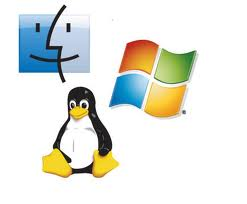
\includegraphics[height=0.22\textheight]{os.png}
			\end{figure}
		\end{column}
		\begin{column}{0.334\textwidth}
			\begin{figure}
				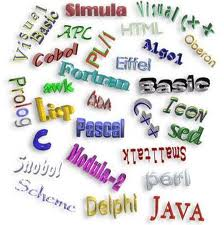
\includegraphics[height=0.22\textheight]{languages_2.png}
			\end{figure}
		\end{column}
		\begin{column}{0.333\textwidth}
			\begin{figure}
				
\includegraphics[height=0.22\textheight]{xml.jpg}
			\end{figure}
		\end{column}
	\end{columns}
	\begin{columns}
		\begin{column}{0.333\textwidth}
			\begin{figure}
				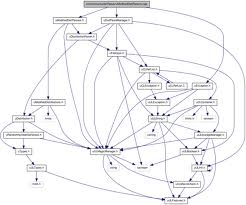
\includegraphics[height=0.22\textheight]{parser.png}
			\end{figure}
		\end{column}
		\begin{column}{0.334\textwidth}
			\begin{figure}
				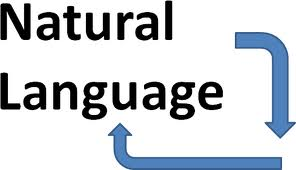
\includegraphics[height=0.22\textheight]{nlp.png}
			\end{figure}
		\end{column}
		\begin{column}{0.333\textwidth}
			\begin{figure}
				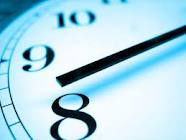
\includegraphics[height=0.22\textheight]{time.png}
			\end{figure}
		\end{column}
	\end{columns}
\end{frame}
% frame_3
\begin{frame}
	\frametitle{New Tool}
	\begin{figure}
		
\includegraphics[height=0.2\textheight]{python_logo.png}
	\end{figure}
\end{frame}
% frame_4
\begin{frame}
	\frametitle{What is Python?}
	\begin{center}
 a remarkably powerful dynamic programming language.
	 \end{center}
		\begin{columns}
		\begin{column}{0.4\textheight}
			\begin{figure}[h]
				\centering
				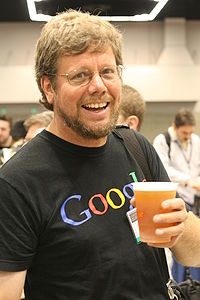
\includegraphics[height=0.5\textheight]{GvR.jpg}
			\end{figure}
		\end{column}
		\begin{column}{0.6\textheight}
			Guido van Rossum\\
			Benevolent Dictator For Life
		\end{column}
	\end{columns}		
\end{frame}
% frame_5
\begin{frame}
	\frametitle{Python's feature}
	\begin{itemize}
		\item free and opensource
			\begin{figure}
				
\includegraphics[height=0.2\textheight]{gnu.png}
				
\includegraphics[height=0.2\textheight]{psf.png}
			\end{figure}
		\item runs everywhere\\
			\begin{columns}
				\begin{column}{0.333\textwidth}
					\begin{figure}
						
\includegraphics[height=0.2\textheight]{linux.png}
					\end{figure}
				\end{column}
				\begin{column}{0.333\textwidth}
					\begin{figure}
						
\includegraphics[height=0.2\textheight]{bsd.png}
					\end{figure}
				\end{column}
				\begin{column}{0.334\textwidth}
					\begin{figure}
						
\includegraphics[height=0.2\textheight]{windows.png}
					\end{figure}
				\end{column}
			\end{columns}
			\begin{columns}
				\begin{column}{0.2\textwidth}
					\begin{figure}
						
\includegraphics[height=0.2\textheight]{mac.png}
					\end{figure}
				\end{column}
				\begin{column}{0.2\textwidth}
					\begin{figure}
						
\includegraphics[height=0.15\textheight]{s60.png}
					\end{figure}
				\end{column}
				\begin{column}{0.2\textwidth}
					\begin{figure}
						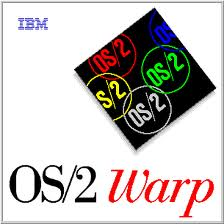
\includegraphics[height=0.15\textheight]{os2.png}
					\end{figure}
				\end{column}
				\begin{column}{0.2\textwidth}
					\begin{figure}
						
\includegraphics[height=0.15\textheight]{vxworks.png}
					\end{figure}
				\end{column}
				\begin{column}{0.2\textwidth}
					\begin{figure}
						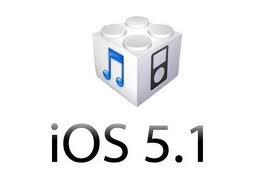
\includegraphics[height=0.15\textheight]{ios.png}
					\end{figure}
				\end{column}

			\end{columns}
	\end{itemize}
\end{frame}
\begin{frame}
	\frametitle{Python's feature}
	\begin{itemize}
		\item plays well with others
			\begin{columns}
				\begin{column}{0.333\textwidth}
					\begin{figure}
						
\includegraphics[height=0.2\textheight]{java.png}
					\end{figure}
				\end{column}
				\begin{column}{0.333\textwidth}
					\begin{figure}
						
\includegraphics[height=0.2\textheight]{dotnet.png}
					\end{figure}
				\end{column}
				\begin{column}{0.333\textwidth}
					\begin{figure}
						
\includegraphics[height=0.2\textheight]{c.png}
					\end{figure}
				\end{column}
			\end{columns}
			\begin{columns}
				\begin{column}{0.3\textwidth}
					\begin{figure}
						
\includegraphics[height=0.2\textheight]{cpp.png}
					\end{figure}
				\end{column}
				\begin{column}{0.3\textwidth}
					\begin{figure}
						
\includegraphics[height=0.2\textheight]{matlab.png}
					\end{figure}
				\end{column}
				\begin{column}{0.4\textwidth}
					\begin{figure}
						
\includegraphics[height=0.2\textheight]{oracle.png}
					\end{figure}
				\end{column}
			\end{columns}
			\begin{columns}
				\begin{column}{0.3\textwidth}
					\begin{figure}
						
\includegraphics[height=0.1\textheight]{fortran.png}
					\end{figure}
				\end{column}
				\begin{column}{0.3\textwidth}
					\begin{figure}
						
\includegraphics[height=0.2\textheight]{CORBA.png}
					\end{figure}
				\end{column}
				\begin{column}{0.4\textwidth}
					\begin{figure}
						
\includegraphics[height=0.2\textheight]{r.png}
					\end{figure}
				\end{column}
			\end{columns}
	\end{itemize}
\end{frame}
% frame_7
\begin{frame}
	\frametitle{Python's feature}
	\begin{itemize}
		\item very clear,readable syntax
		\begin{figure}
			\scriptsize{Implementing the basic QuickSort algorithm in Python}
			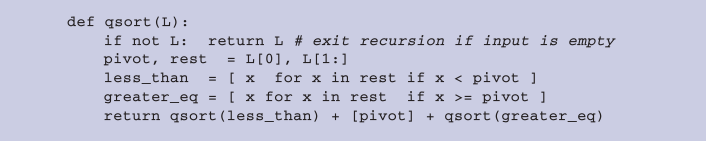
\includegraphics[height=0.22\textheight]{quick_sort.png}\\
		\end{figure}
	    \item Mandatory indentation
	\end{itemize}
	\begin{itemize}
		\item boosts developer productivity\\
			Python code is typically $\frac{1}{3}$ to $\frac{1}{5}$ the size of
			equivalent C++ or Java code.
	\end{itemize}
\end{frame}
% frame_8
\begin{frame}
	\begin{figure}
		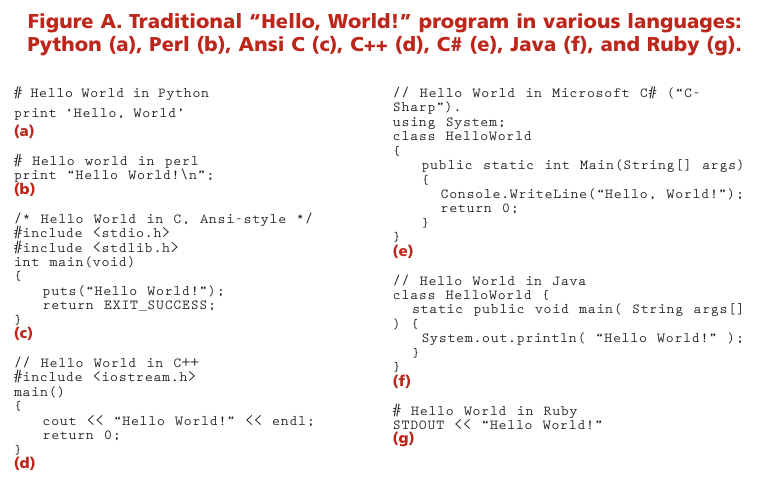
\includegraphics[height=0.7\textheight]{hello_world.png}
	\end{figure}
\end{frame}
% frame_9
\begin{frame}
	\frametitle{How to replace Matlab?}
	\framesubtitle{Python:An Ecosystem for Scientific Computing}
	\begin{figure}
		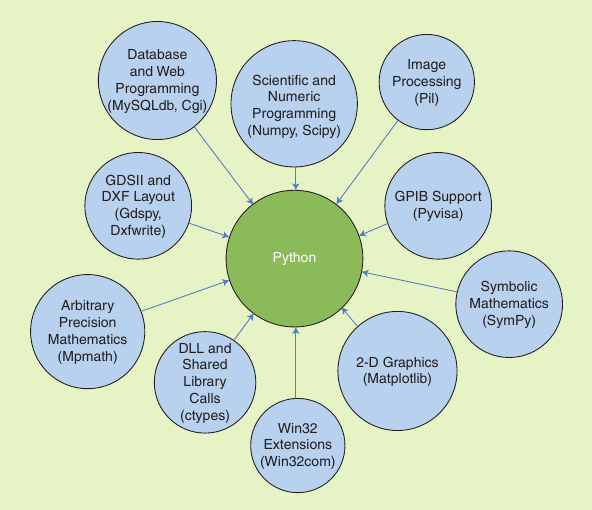
\includegraphics[height=0.8\textheight]{python_1.png}
	\end{figure}
\end{frame}
% frame_10
\begin{frame}
	\frametitle{NumPy}
	\framesubtitle{N-dimensional Array manipulations}
	\begin{columns}
		\begin{column}{0.5\textwidth}
			\begin{itemize}
				\item N-dimensional array object
			\end{itemize}
			\begin{figure}
				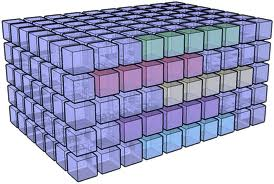
\includegraphics[height=0.2\textheight]{ndarray.png}
			\end{figure}
		\end{column}
		\begin{column}{0.5\textwidth}
			\begin{itemize}
				\item linear algebra functions
			\end{itemize}
			\begin{figure}
				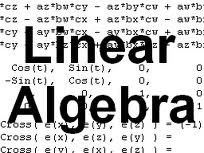
\includegraphics[height=0.2\textheight]{linear_algebra_1.png}
			\end{figure}
		\end{column}
	\end{columns}
	\begin{columns}
		\begin{column}{0.5\textwidth}
			\begin{itemize}
				\item Fourier transforms
			\end{itemize}
			\begin{figure}
				
\includegraphics[height=0.3\textheight]{fft.png}
			\end{figure}
		\end{column}
		\begin{column}{0.5\textwidth}
			\begin{itemize}
				\item random number capabilities
			\end{itemize}
			\begin{figure}
				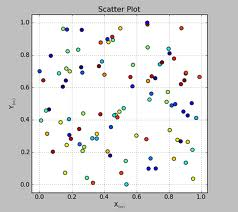
\includegraphics[height=0.3\textheight]{random.png}
			\end{figure}
		\end{column}
	\end{columns}
\end{frame}
\begin{frame}
	\frametitle{SciPy}
	\framesubtitle{Scientific tools for Python}
	\begin{columns}
		\begin{column}{0.5\textwidth}
			\begin{center}
				a library of scientific tools  \\
				depends on the NumPy 
			\end{center}
		\end{column}
		\begin{column}{0.5\textwidth}
			\begin{figure}
				
\includegraphics[height=0.3\textheight]{scipy.png}
			\end{figure}
		\end{column}
	\end{columns}
	SciPy provides moudles for
	\begin{columns}
		\begin{column}{0.5\textwidth}
			\begin{itemize}
				\item statistics\\
				\item optimization\\
				\item numerical integration\\
				\item linear algebra\\
				\item Fourier transforms
			\end{itemize}
		\end{column}	
		\begin{column}{0.5\textwidth}
			\begin{itemize}
				\item signal processing\\
				\item image processing\\
				\item ODE solvers\\
				\item special functions 
				\item ...
			\end{itemize}
		\end{column}
	\end{columns}
\end{frame}

% frame_12
\begin{frame}
	\frametitle{Image Processing}
	\begin{columns}
		\begin{column}{0.1\textwidth}
			\begin{itemize}
				\item PIL
			\end{itemize}
		\end{column}
		\begin{column}{0.9\textwidth}
			\begin{figure}
				
\includegraphics[height=0.3\textheight]{pil.png}
				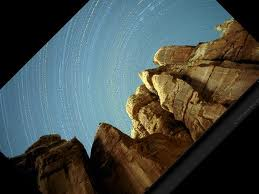
\includegraphics[height=0.3\textheight]{pil_1.png}
			\end{figure}
		\end{column}
	\end{columns}
	\begin{columns}
		\begin{column}{0.2\textwidth}
			\begin{itemize}
				\item pyopencv
			\end{itemize}
		\end{column}
		\begin{column}{0.4\textwidth}
			\begin{figure}
				
\includegraphics[height=0.3\textheight]{opencv.png}
			\end{figure}
		\end{column}
		\begin{column}{0.4\textwidth}

			\begin{figure}
				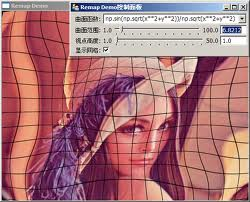
\includegraphics[height=0.3\textheight]{pyopencv.png}
			\end{figure}
		\end{column}
	\end{columns}
\end{frame}
% frame_13
\begin{frame}
	\frametitle{SymPy}
	\begin{columns}
		\begin{column}{0.5\textwidth}
			\begin{center}
				SymPy is a Python library for symbolic mathematics.
			\end{center}
		\end{column}
		\begin{column}{0.5\textwidth}
			\begin{figure}
				
\includegraphics[height=0.3\textheight]{sympy.png}
			\end{figure}
		\end{column}
	\end{columns}
	SymPy provides moudles for 
	\begin{columns}
		\begin{column}{0.5\textwidth}
		\begin{itemize}
			\item Core capabilities
			\item Polynomials
			\item Calculus
			\item Solving equations
			\item Discrete math
			\item Matrices
		\end{itemize}
	\end{column}
	\begin{column}{0.5\textwidth}
		\begin{itemize}
			\item Geometric Algebra
			\item Geometry
			\item Plotting
			\item Physics
			\item Statistics
			\item Printing
		\end{itemize}
	\end{column}
\end{columns}
\end{frame}
% frame_14
\begin{frame}
	\frametitle{matplotlib}
	\framesubtitle {a python 2D plotting library}
	matplotlib is Object-Oriented and its syntax looks like matlab's.\\
	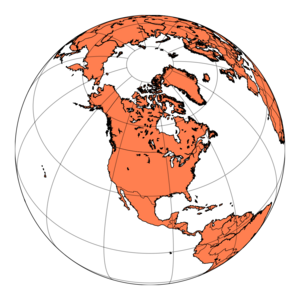
\includegraphics[height=0.5\textheight]{matplotlib_2.png}
	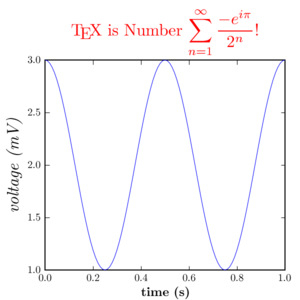
\includegraphics[height=0.5\textheight]{matplotlib_1.png}\\
	Tips:It is neccessary to get a handle on its inheritance relationship.
\end{frame}
% frame_15
\begin{frame}
	\frametitle{Mayavi Project}
	\framesubtitle{3D Scientific Data Visualization and Plotting}
	\begin{columns}
		\begin{column}{0.5\textwidth}
			The Mayavi project includes two related packages for 3-dimensional
			visualization:
			\begin{itemize}
				\item Mayavi: A tool for easy and interactive visualization of
					data, with seamless integration with Python scientific
					libraries.
				\item TVTK: A Traits-based wrapper for the Visualization
					Toolkit, a popular open-source visualization library.
			\end{itemize}
		\end{column}
		\begin{column}{0.5\textwidth}
			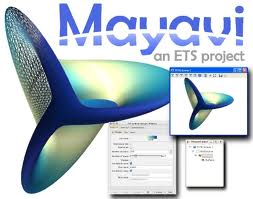
\includegraphics[height=0.4\textheight]{mayavi_1.png}
		\end{column}
	\end{columns}
\end{frame}
% frame_16
\begin{frame}
	\frametitle{MayaVi Screenshots}
	\begin{columns}
		\begin{column}{0.5\textwidth}
			\begin{figure}
				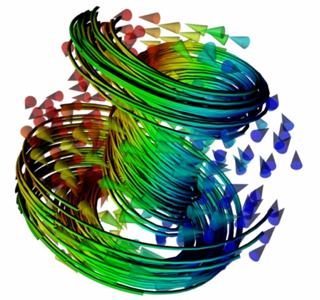
\includegraphics[height=0.35\textheight]{mayavi-samp.png}
			\end{figure}
		\end{column}
		\begin{column}{0.5\textwidth}
			\begin{figure}
				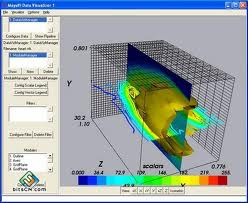
\includegraphics[height=0.35\textheight]{mayavi_9.png}
			\end{figure}
		\end{column}
	\end{columns}
	\begin{columns}
		\begin{column}{0.5\textwidth}
			\begin{figure}
				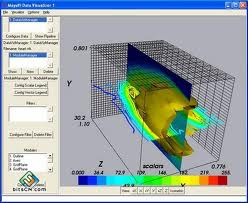
\includegraphics[height=0.35\textheight]{mayavi_8.png}
			\end{figure}
		\end{column}
		\begin{column}{0.5\textwidth}
			\begin{figure}
				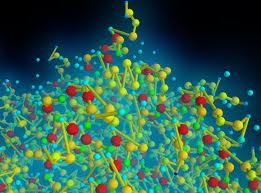
\includegraphics[height=0.35\textheight]{mayavi_7.png}
			\end{figure}
		\end{column}
	\end{columns}
\end{frame}
% frame_17
\begin{frame}
	\frametitle{GUI Programming}
	\begin{columns}
		\begin{column}{0.2\textwidth}
			\begin{itemize}
				\item PyQt
			\end{itemize}
		\end{column}
		\begin{column}{0.4\textwidth}
			\begin{figure}
				\includegraphics[height=0.3\textheight]{pyqt.png}
			\end{figure}
		\end{column}
		\begin{column}{0.4\textwidth}
			\begin{figure}
				\includegraphics[height=0.3\textheight]{pyqt.jpg}
			\end{figure}
		\end{column}
	\end{columns}
	\begin{columns}
		\begin{column}{0.2\textwidth}
			\begin{itemize}
				\item wxPython
			\end{itemize}
		\end{column}
		\begin{column}{0.4\textwidth}
			\begin{figure}
				\includegraphics[height=0.3\textheight]{wxPython.png}
			\end{figure}
		\end{column}
		\begin{column}{0.4\textwidth}
			\begin{figure}
				\includegraphics[height=0.3\textheight]{wxpython_1.png}\\
			\end{figure}
		\end{column}
	\end{columns}
	\begin{flushleft}
	Tkinter PyGtk PyGUI PyKDE ...
\end{flushleft}
\end{frame}
% frame_18
\begin{frame}
	\frametitle{PyPy}
	\framesubtitle{the coming future}
	PyPy is a fast, compliant alternative implementation of Python.\\
	It has several advantages and distinct features:
	\begin{columns}
		\begin{column}{0.6\textwidth}
			\begin{itemize}
				\item Much faster speed(thanks to JIT)
				\item Less memory usage 
				\item Highly compatible
				\item Sandboxing
				\item Stackless
			\end{itemize}
		\end{column}
		\begin{column}{0.4\textwidth}
			\begin{figure}
				\includegraphics[height=0.4\textheight]{pypy.png}
			\end{figure}
		\end{column}
	\end{columns}
\end{frame}
% frame_19
\begin{frame}
	\frametitle{How fast is PyPY?}
	\begin{figure}
		\includegraphics[height=0.65\textheight]{fast_pypy_1.png}
	\end{figure}
	\tiny{It depends greatly on the type of task being performed. The geometric
	average of all benchmarks is 0.19 or 5.4 times faster than CPython}
\end{frame}
% frame_20
\begin{frame}
	\frametitle{PyPy is evolving}
	\begin{figure}
		\includegraphics[height=0.65\textheight]{pypy_evolving.png}
	\end{figure}
\end{frame}
		
% frame_18
\begin{frame}
	\frametitle{Summary}
	an efficient frame for scientific computing
	\begin{figure}
		\includegraphics[height=0.3\textheight]{summary.png}
	\end{figure}
\end{frame}
\end{document}
